\begin{doublespace}
\chapter{Tax planning and BEPS: a transportation model for optimal profit allocation}
This chapter deals with the problem of multinational entity allocation based on three main factors, namely the costs, the tax pressure and the functional characterization of a certain entity. The solution suggested is a goal programming model that embeds this limitation imposed by the environment and tries to find an optimal solution that permits the Decision Maker to be competitive \textit{vis-à-vis} multinational competitors. The results obtained from such model are many times different from the ones putted into places by multinationals, which tend to focus on minimizing only the tax base without taking into account other information that may result in significant value added from a tax planning perspective. 

\section{Introduction}
After the Great Recession, multinational companies found themselves in a very different environment; thriving to survive with competition on one side and higher restriction imposed by countries running financial crises. This led multinationals with a great challenge which consequently boost cost engineering, in an attempt to survive in this new scenario. Another result was a new form of tax planning, most of the time barely legal in order to exploit the fiscal advantages of certain countries\cite{After_tax_hedging_report_2013}. Such problems forced the G20 to launch an inclusive framework on base erosion and profit shifting called "BEPS", bringing together about 100 countries in order to stop such unlawful tax planning. However, even if this action against such problem highlighted in a more specific way what should be considered as aggressive tax planning the border with legitimate cost engineering seems blurrier than ever\cite{Feller2017}.

In this paper, is proposed Goal Programming model, Figure\ref{fig:flowchart}, that given a set of criteria based on the accounting information of a specific multinational, it tries to perform the best allocation of its entities. The model will use both internal and external data and will follow three main objectives, namely minimize the costs, minimize the tax base and at the same time be compliant with the functional characterization of each and every entity constituting the multinational group. In other words the last objective impose that the multinational entity profitability has to be in line with independent actor in the market\cite{Model_Tax_Convention_2015} and should not be in any case a mere result of aggressive tax planning.

\begin{figure}
\centering
\begin{tikzpicture}[
squarednode/.style={rectangle, draw=black!60, minimum height=10mm, minimum width=40mm},
circlenode/.style={circle, draw=black!60, minimum size=5mm},
blanknode/.style={rectangle, draw=white!60, minimum height=0mm, minimum width=10mm}
]

\node[circlenode]      (maintopic)                              {GP Model};
\node[blanknode]        (b1)       [left=of maintopic] {};
\node[blanknode]        (b2)       [left=of b1] {};
\node[squarednode]        (t1)       [above=of maintopic] {Target enterprise data};
\node[squarednode]      (t2)       [right=of maintopic] {Optimal allocation};
\node[squarednode]        (t3)       [above=of b2] {Global enterprises data};
\node[squarednode]        (t4)       [below=of b2] {Macroeconomic data};

\draw[->] (t1.south) -- (maintopic.north);
\draw[->] (t4.east) -- ++ (0.45cm,0) |- (maintopic.west);
\draw[->] (t3.east) -- ++ (0.45cm,0) |- (maintopic.west);
\draw[->] (maintopic.east) -- (t2.west);
\end{tikzpicture}
\caption{Model flowchart}
\label{fig:flowchart}
\end{figure}

The following paper is organized in five sections, apart from the first one which focuses on giving a brief introduction to the topic that is going to be addressed and modelled; the last chapters will be stand-alone sections developing specific parts of the process of model formulation and analysis. Specifically at section two is given an extensive overview of the set of approaches dealing with multi-criteria decision analysis; in particular in this section will be given a theoretical overview of the main categories of multi-criteria analysis and will be further developed the concept of Goal Programming in its common formulation, namely lexicographic, weighted and min-max or Chebyshev Goal Programming. After this high level overview the focus will be set to the goal programming itself and a state-of-the-art review will be given, in order to give a pragmatic point of view to the new development to in the field the state-of-the-art review will take into account three main area of application, and then the focus will be oriented to the cross field of accounting, which is the one where the model belongs. Concluded this overview the formulation of the model will start from the data gathering process, the data will be categorized in three different typologies as highlighted by the flowchart in figure \ref{fig:flowchart}. After the process of data gathering, the full model will be formulated in a goal programming fashion defining, objectives, soft constraints and hard constraints.
\\
\\
Ultimately the model will be run using the LINGO software package. The weights used will be subjected by a sensitivity analysis through different scenarios. Then, a set of weights will be chosen to take into account the decision maker preferences and the results will be compared with the real result obtained by the company in the period under scope, in doing so some limitations of the model will be stated and further analyzed.

\pagebreak 
\section{Multi-criteria decision analysis}
Even if the practice of decision-making is old as man, academics tend to date the roots of modern MCDA in the early 60s, where the focus at the time was to find the most preferred solution, or generating an approximation to the entire efficient frontier\cite{Greco2016}.
\\
Multi-criteria analysis may be defined as a problem of multiple-objective programming, that differs from a linear one,
since more objective function are handled; its formulation is the following:
	$$
	Min[f_1(x),f_2(x),...,f_k(x)] \quad i=1,...,k \quad where \quad k\geq2
	$$
This approach seems to fit better the real world since, in reality, more than one objective is pursued, and most of the time in contrast with one another.
A solution to a multi-criteria problem would be optimal if it'd respected the Pareto Efficient assumption, namely that no other feasible solution exists that is at least as good with respect to all objectives and strictly better with respect to at least one objective. Mathematically it means that $\left\{x_1,...x_k\right\}$ is a solution if $\not\exists \left\{x'_1,...x'_k\right\}$
such that:
	\[
	g(f_1(x),f_2(x),...,f_k(x)) \leq g(f_1(x'),f_2(x'),...,f_k(x')) \quad \forall n \quad \in  \left\{1...k\right\}
	\]
However such increase in complexity given by multiple objectives is both the strength and the weakness of such methodology, this is due to the fact that we have to deal with $N$ trade-offs deriving from the objectives we decided to include in our optimization problem. Because of this problem a lot of approaches and specific intelligent algorithms were proposed\cite{Cui2017}.

Focusing the attention on the approaches suggested, four main categories emerge, namely:

\begin{itemize}
	\item A Priori methods: such methods are characterized by prior definition of the preference information, this category includes methods such as Weighted Sum Method, Constraints Method, Objective Programming Method, Dictionary Ordering Method and Analytic Ordering Method;   
	\item Interactive methods: in this particular category the process is iterative, meaning that the decision maker interacts with the preference information he gave in search of the optimal solution, from this category belong two types of methods namely the Normal Boundary Intersection and the Normalized Normal Constraint;
	\item Pareto-dominated methods: these methods divides the optimal solution seeking in two parts, at first they try to compose the efficient frontier of a given multi-criteria problem, then they try to find the Pareto Dominant\footnote{Given a vector of outcomes $\vec{S}$ that we identified as the Efficient Frontier $\vec{S}[s_1..._n]$ a solution $s^{\star}$ of such vector is Pareto Dominant if $\nexists$ a $s_q$ that is Pareto superior to $s^{\star}$.} solution;
	\item New Dominance methods: this methods may be considered as an extension of the Pareto-dominated methods, in that they try to build the efficient frontier, then they try to eliminate the Pareto-dominated solutions however they tend to use fuzzy methods and other solutions to avoid the computational drawback of the former one.  
\end{itemize}

From the set of the A Priori methods belongs the Goal Programming (which develops from the concept of linear programming) and will be used to model the problem of entities allocation proposed on the next chapters.
\\
Goal Programming, hereinafter GP, is a multi-criteria decision analysis approach which allows the decision maker to consider simultaneously several conflicting objectives.

The idea behind such method is very simple, and is based on distance minimization; this means that at each objective function is associated a deviation variable that has to be minimized in batch with the other deviation variables coming from the other objective functions.

Such models may be represented algebraically as follows:

\begin{equation*}
\begin{aligned}
& \underset{n,p}{\text{minimize}}
& & a=h(n,p) \\
& \text{subject to}
& & f_q(x)+n_q-p_q=b_q \\
& & & x\in F \\
& & & n_q,p_q\geq 0 
\end{aligned}
\end{equation*}

GP is vastly applied in many sciences\cite{Tamiz1998}. Its origins are dated back to the 50s, firstly introduced by Abraham Charnes and William Cooper\cite{Charnes1955} with an article on the optimal estimation of executive compensation.

In such approach, three main different categories have been identified, namely the lexicographic GP, the weighted GP and the Chebyshev GP.

Lexicographic GP, also named “preemptive” Goal Programming, distinguish itself from the other GP techniques as it has a number of priority levels chosen a priori. The mathematical formulation is the following one:

\begin{equation*}
\begin{aligned}
& \underset{n,p}{\text{Lex minimize}}
& & [h_1(n,p),...,h_L(n,p)] \\
& \text{subject to}
& & f_q(x)+n_q-p_q=b_q, \; q=1,...Q \\
& & & x\in F \\
& & & n_q,p_q\geq 0, \; q=1,...,Q 
\end{aligned}
\end{equation*}

As opposed to LGP, the WGP allows for direct trade-offs between all unwanted deviational variables by using weight that are not putted a priori (as the LGP), as a result WGP is more flexible but as counter-effect it requires more computational power. The mathematical formulation is the following one:

\begin{equation*}
\begin{aligned}
& \underset{n,p}{\text{minimize}}
& & \sum_{q=1}^{Q}(\frac{u_q n_q}{k_q}+\frac{v_q n_q}{k_q}) \\
& \text{subject to}
& & f_q(x)+n_q-p_q=b_q, \; q=1,...Q \\
& & & x\in F \\
& & & n_q,p_q\geq 0, \; q=1,...,Q 
\end{aligned}
\end{equation*}

The last GP variant, presented by Flavell. It differs from the first two variants since it uses the underlying $ L_\infty $ means of measuring distance. Also, called Minmax goal programming it seeks to minimize the maximal deviation from any goal. Therefore, the primary goal of such approach is the balance. The mathematical formulation is the following one:

\begin{equation*}
\begin{aligned}
& \underset{\lambda}{\text{minimize}}
& & \lambda \\
& \text{subject to}
& & \frac{u_q n_q}{k_q}+\frac{v_q n_q}{k_q}\leq\lambda, \; q=1,...Q \\
& & & f_q(x)+n_q-p_q=b_q, \; q=1,...Q \\
& & & x\in F \\
& & & n_q,p_q\geq 0, \; q=1,...,Q 
\end{aligned}
\end{equation*}

\pagebreak 

\section{A state-of-the-art review: Goal Programming}
The Goal Programming is probably one of the most used tool by academics and practitioners in solving multi criteria optimization problems, even though such preferences do not follow a linear path\cite{Romero2014}\cite{Schniederjans1995}. The main field of research and application of the Goal Programming are undoubtedly three, namely engineering, social sciences and management\cite{Colapinto2017a}, with the former one leading for the number of its applications.
Especially in engineering the GP techniques used the most are the ones involving hybrid techniques (combining multiple different GP approaches) and Fuzzy Goal Programming (FGP) The models proposed tackle macro-areas such as supply chain and logistics management, with problems involving closed loop supply chain, dealing with the treatment and recycling activities\cite{Zarandi2011}. 
\\
Quite the opposite occur in the applications of social sciences field, where, in the majority of the case to the field of economics. The last research in which is reported the use of Goal Programming was inherent the sub field of macroeconomics, analyzing the nature of the inter generational equity and sustainable development in order to understand how the players involved can achieve their aim of maximizing social welfare in the short run without compromising the future possibilities. In the case of social science the most used approaches are the plain vanilla ones of GP, ranging from lexicographic GP to weighted GP.
\\
Lastly the management field which accounts for a great number of applications, especially in the field of strategic management, portfolio selection and marketing where there is a great diversity between techniques that ranges from fuzzy sets\cite{Trenado2014} to weighted goal programming and hybrid approaches.
\\
All the three fields proposed when applied in modeling corporation have a common backbone (as exposed by Figure \ref{fig:accounting})  in which they gather information which is called accounting; embracing significant development particularly in areas dealing with, cost controlling, budgeting and operations planning; such cross literature will be treated in the following section.

\begin{figure}
\begin{center}
\begin{tikzpicture}
    \draw \firstcircle node[above] {Engineering};
    \draw \secondcircle node [above] {Social sciences};
    \draw \thirdcircle node [above] {Management};
    \draw \fourthcircle node [above] {Accounting};

    \begin{scope}
      \clip \fourthcircle;
      \fill[gray, fill opacity=0.5] \firstcircle;
       \clip \fourthcircle;
      \fill[gray, fill opacity=0.5] \secondcircle;
      \clip \fourthcircle;
      \fill[gray, fill opacity=0.5] \thirdcircle;
      \end{scope}

\end{tikzpicture}
\end{center}
\caption{The meddling of accounting in the three main field of application of Goal Programming} \label{fig:accounting}
\end{figure}

\subsection{Application in Accounting}
The accounting field (where the model proposed belongs), as seen in the following year a brand-new interest among researchers. It's worth starting by defining what is meant for accounting, which may be defined as the process of recording and summarizing business and financial transactions, analyzing and reporting the results. Although this seems as passive process, sometimes accounting has reveled to be a very strong tool on the hands of the decision maker\cite{Davidson1961} to enact decision in the most informed way possible. In fact, because of the nature of accounting which may be seen as a cross organizational field, the DM has the possibility to test particular strategies having a series of objectives belonging from different departments, from the legal to the marketing and from the logistic to the production department.

In such situation the GP may turn out to be a very powerful tool, as highlighted by Aouni\cite{Aouni2017}; generally accountants are facing complex decision-making situations where they aggregate simultaneously several conflicting and incommensurable factors. Given this situation a multi criteria analysis tool is, without any doubt the best fit approach possible and GP turns out to be used as framework because of its simplicity of formulation and at the same time the power of the flexibility that it provides. In the following table is proposed a review of the brand-new articles written in the field and their main contribution.

\begin{center}
\begin{tabular}{ || m{11em} m{20em}|| }
 \hline
 Author & Novelty \\ 
\hline\hline
Ijiri and Kaplan\cite{Ijiri1971} & The authors propose a weighted approach to set a perfect sampling policy in auditing according to four objectives, namely: representative, corrective, protective and preventive sampling. \\
\hline
Tayi and Gangolly\cite{Tayi1985} & The authors, building on what proposed in the filed of audit sampling, propose instead of a weighted GP, a sapling based on a new approach, namely a polynomial GP which guarantees a better contemplation of the trade-offs between objectives. \\
\hline
Killough and Souders\cite{Killough1973} & The authors apply the GP in the field of audit staff planning for public accounting firms distinguishing between role and chargeable hours. \\
\hline
Welling\cite{Welling1977} & The author proposes a GP approach to solve the problem of human resource evaluation using non monetary based parameters. \\
\hline
Krüger and Hattingh\cite{Kruger2006} & The authors propose a combination of Analytic Hierarchy Process and Goal Programming in order to address the risk of allocating the hours on several projects. \\
\hline
Gardner et al.\cite{Gardner1990} & The authors use a multi period approach to audit the staff planning through a series of objectives, namely, profit, late completion of work, work declined, staff augmentation, staff reduction, under utilization of the work force, and shortfall in meeting professional development targets. \\
\hline
Kwak et al.\cite{Kwak2003} & The authors propose one of the first multiple-objective auditing model, combining strategic objectives and human resources allocation using fuzzy set. \\
\hline
Zamfirescu and Zamfirescu\cite{Zamfirescu2013} & The authors apply a lexicographic goal programming to enact a performance based budgeting(PBM) on funds allocation in a real public company. \\
\w
Tan et al.\cite{Tan2008} & The authors propose a GP model in order to help contractors to decide the optimal level of resources to be consumed within a set of limitations.  \\
\hline 
Iranmanesh and Thomson\cite{Iranmanesh2008} & The authors develop a model for product design based
on quality function deployment (QFD) whose aim is to optimize cost and design characteristics during product
development. \\
 \hline\end{tabular}
\end{center}

From such table is possible to see how many GP models have been created to solve a broad range of accounting topics such as in audit sampling or other fields dealing with management accounting such as pricing, costing, capital budgeting and performance evaluation.
This popularity is due to the fact that GP is easy to understand and to apply, plus it facilitates consideration of trade-off in the decision-making process which is perceived a by the authors proposed as a deal-breaker when facing the decision on whether to use a GP approach.
\\
However it's worth mentioning the fact that not every field of accounting gained the same attention by both researchers and practitioner and, aside from its popularity, the interest in international tax planning never arose. This may be due to the typical background that such researchers have on the field. In fact most of the research moved in this field pertain to the legal area, which probably lack from a point of view of mathematical modelling skills. From the other side the field of international taxation involves a great set of laws, both soft and hard, that may result in a great effort by practitioner to model. 
From an extensive review of the field of study under scope, it’s worth mentioning the work of Merville and Petty\cite{Merville1978} who tried to model an optimal pricing policy which is indeed useful to set a global tax strategy since the TP core is base on that. However, one major problem of such model is given by the fact that it doesn't take into account the novelties introduced by the recent work of the OECD and the increasing importance of new tools at the disposal of multinational companies such as: extensive databases, and newer resource management tools.
\\
Therefore, keeping what proposed by the literature, seems necessary to propose a new type of model which takes into account these new developments and result giving a powerful tool in the hand of the Decision Maker.

\pagebreak

\section{Model formulation}

\subsection{Data used to formulate the model}
The data used in this particular GP model comes from different sources, and they can be summarized in the following categories:
\begin{itemize}
    \item Macroeconomic data, is the set of data used by DM that came from the national economies;
    \item Target enterprise data, are the types of data that refer particularly to the firm under scope;
    \item Global enterprises data, these data comes from other enterprises that are in some way similar to the enterprise under scope, both in terms of business or because of the functions they perform.
\end{itemize}

\subsubsection{Macroeconomic data}
The group of Macroeconomic data includes the Corporate Tax Rate defined as "the percentage on corporate income generated deemed to the State". The Figure 2 below shows how this rate is different from State to State. This means that different allocation of corporate entities may result in an advantage from a competitive perspective. For example, a new allocation from Germany to Estonia may result in a gain in terms of income of +30\% on net income that may be reinvested in the company.
\begin{figure}
\centering
  \centering
  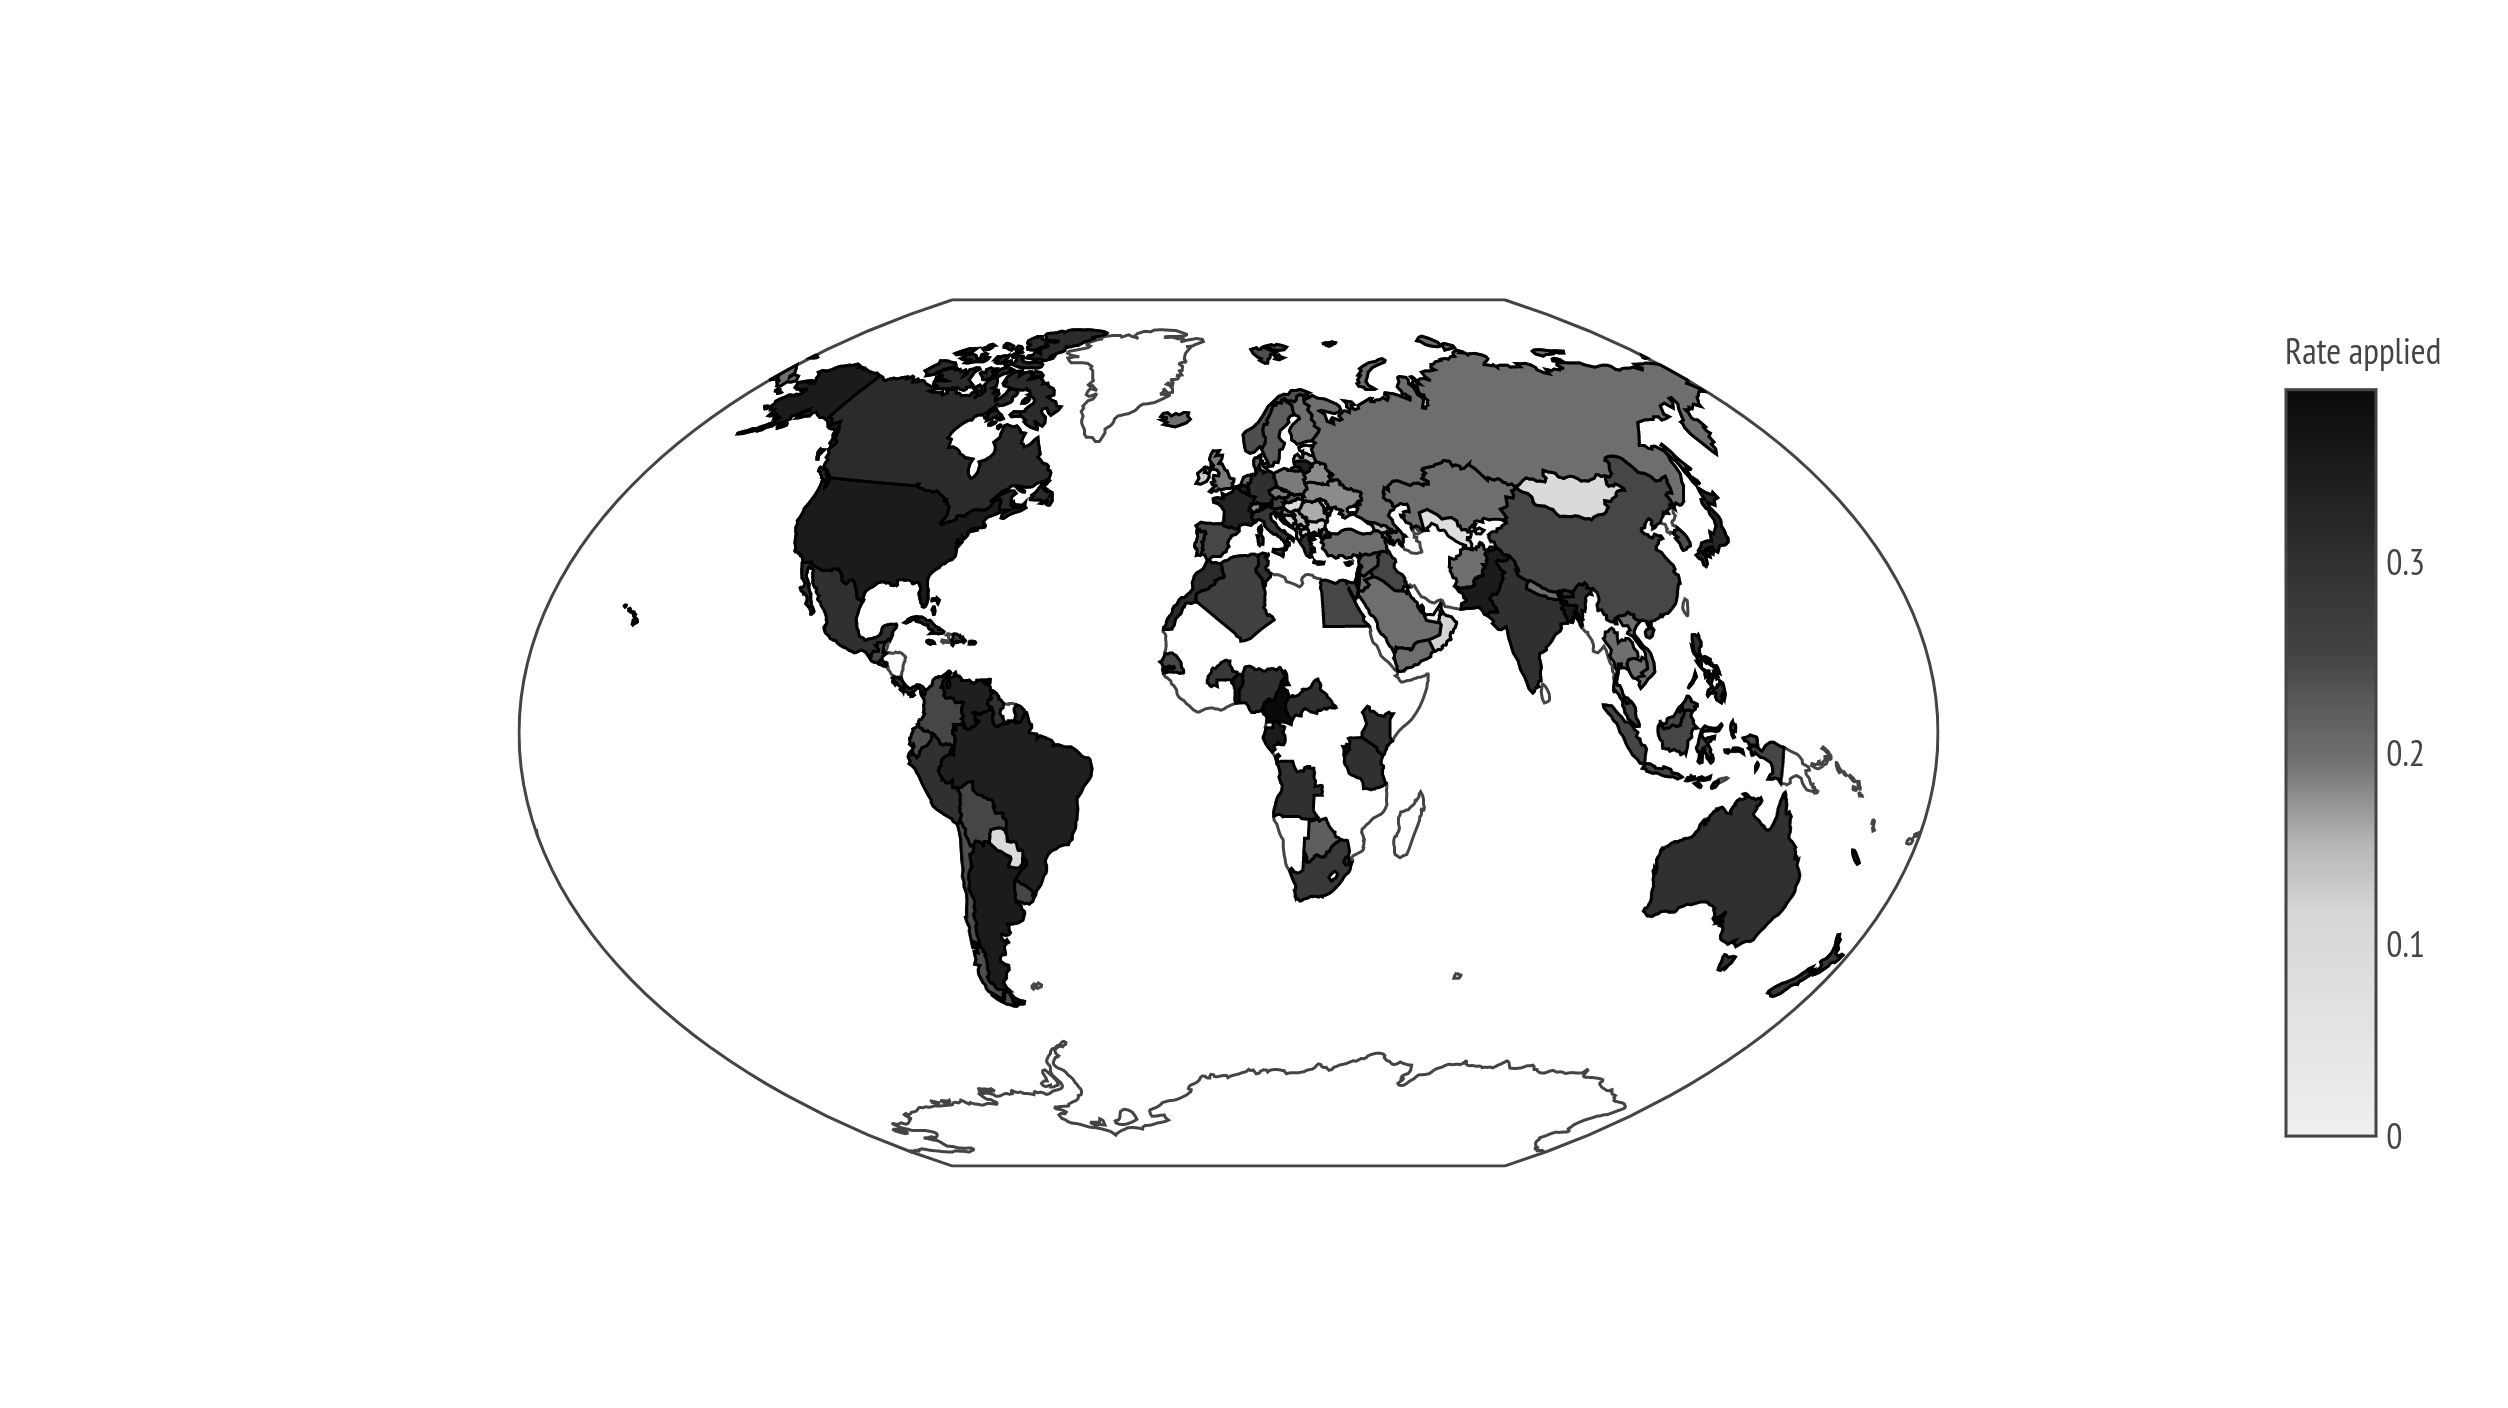
\includegraphics[width=1\linewidth]{Images/CTworld.png}
  \caption{Corporate Tax around the world}
  \label{fig:test1}
\end{figure}

The second Macroeconomic data is the Gross National Income per Capita. This kind of index is a good proxy for the average cost of an employee per year which instead is computed by dividing the national-accounts-based total wage bill by the average number of employees in the total economy, which is then multiplied by the ratio of the average usual weekly hours per full-time employee to the usually average weekly hours for all employees. The latter indicator was not chosen since it computed in very few countries (the OECD countries) and doesn't permit to obtain a full range of choice by the model. Figure 3 reported below shows the geographical distribution of such index from state to state.
\begin{figure}
  \centering
  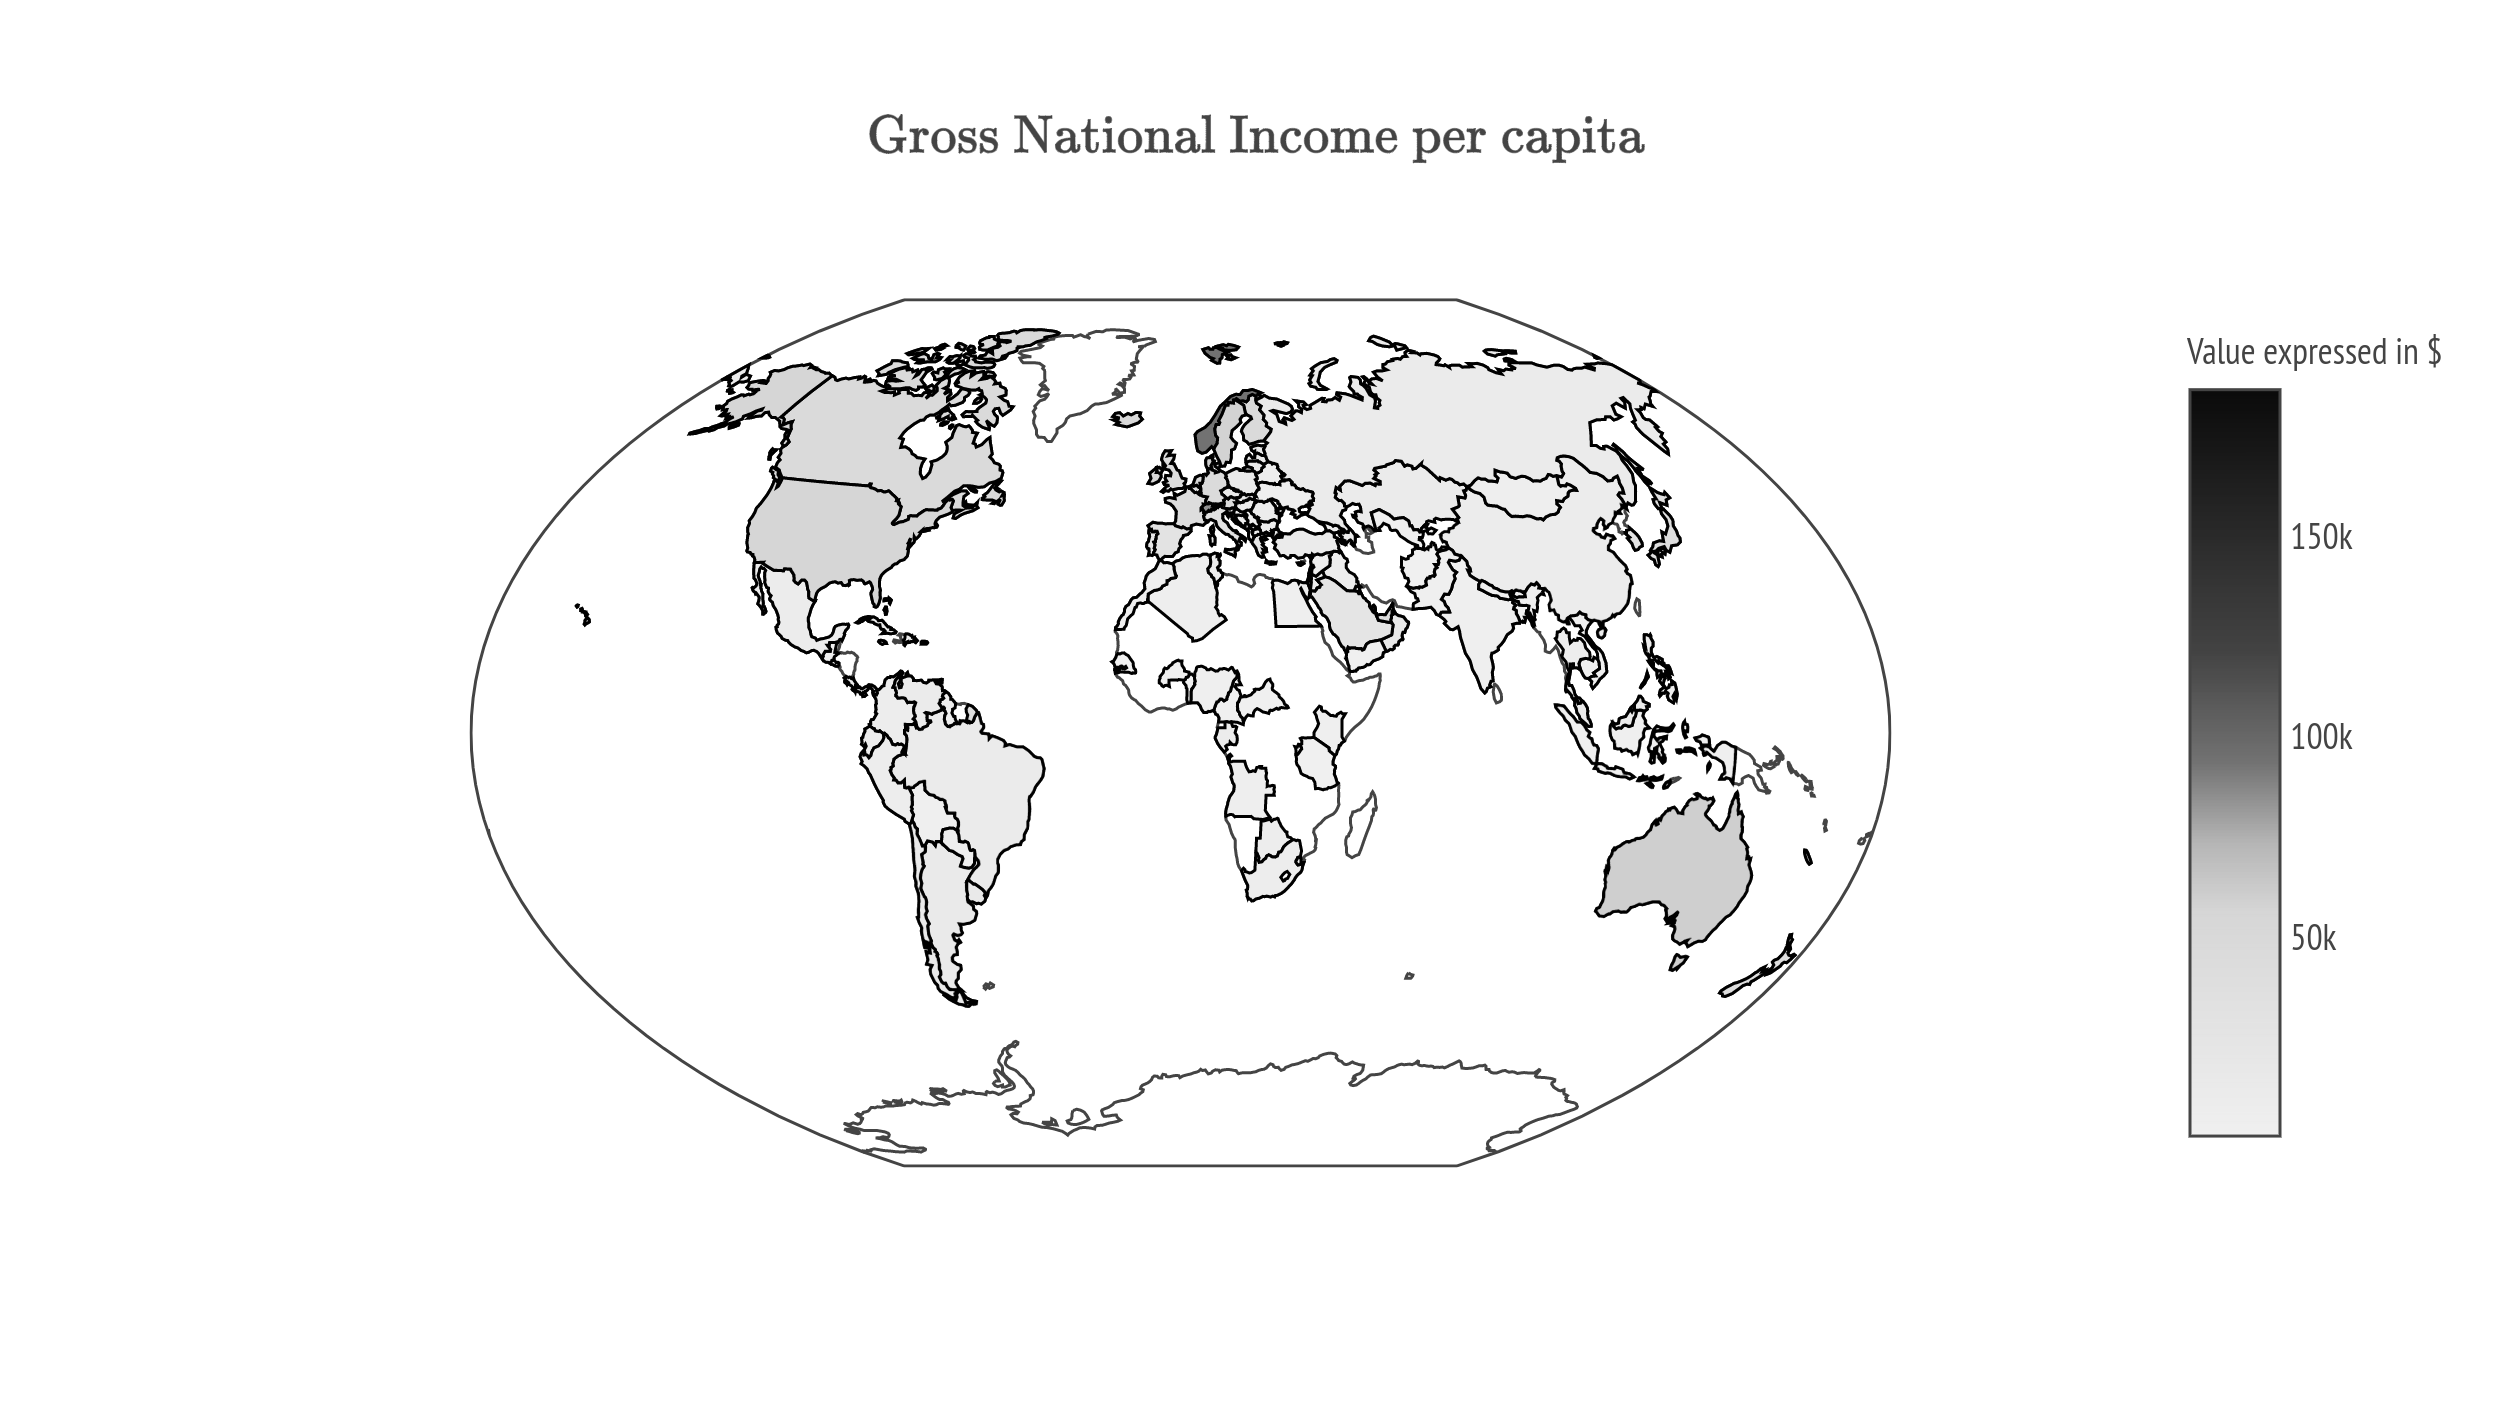
\includegraphics[width=1\linewidth]{Images/GNIworld.png}
  \caption{Gross National Income per Capita}
  \label{fig:test2}
\end{figure}

Figure 4 shows a scatter plot of the normalized Corporate Tax (x-axis) and GNI per Capita (y-axis), to such data a  K-mean cluster algorithm with K=5 was applied; this kind of algorithm randomly assigns each observation to a cluster, and finds the centroid of each cluster then, through iteration reassign data points to the cluster whose centroid is closest and calculate the new centroid of each cluster. The K was chosen with the "elbow method" with $R^2$ meaning that 5 was the number of cluster that return the best trade off in terms of $R^2$ increase and cluster numerosity.
The result were five clusters with the one highlighted by the circle indicating countries with both a low average cost of worker and a low taxation. However, even if these may seem the best locations to allocate the entities this is not always true, since the formula for taxation is the one proposed at section 4.2 and such entities have to be in the range proposed in section 4.3.

\begin{figure}
\centering
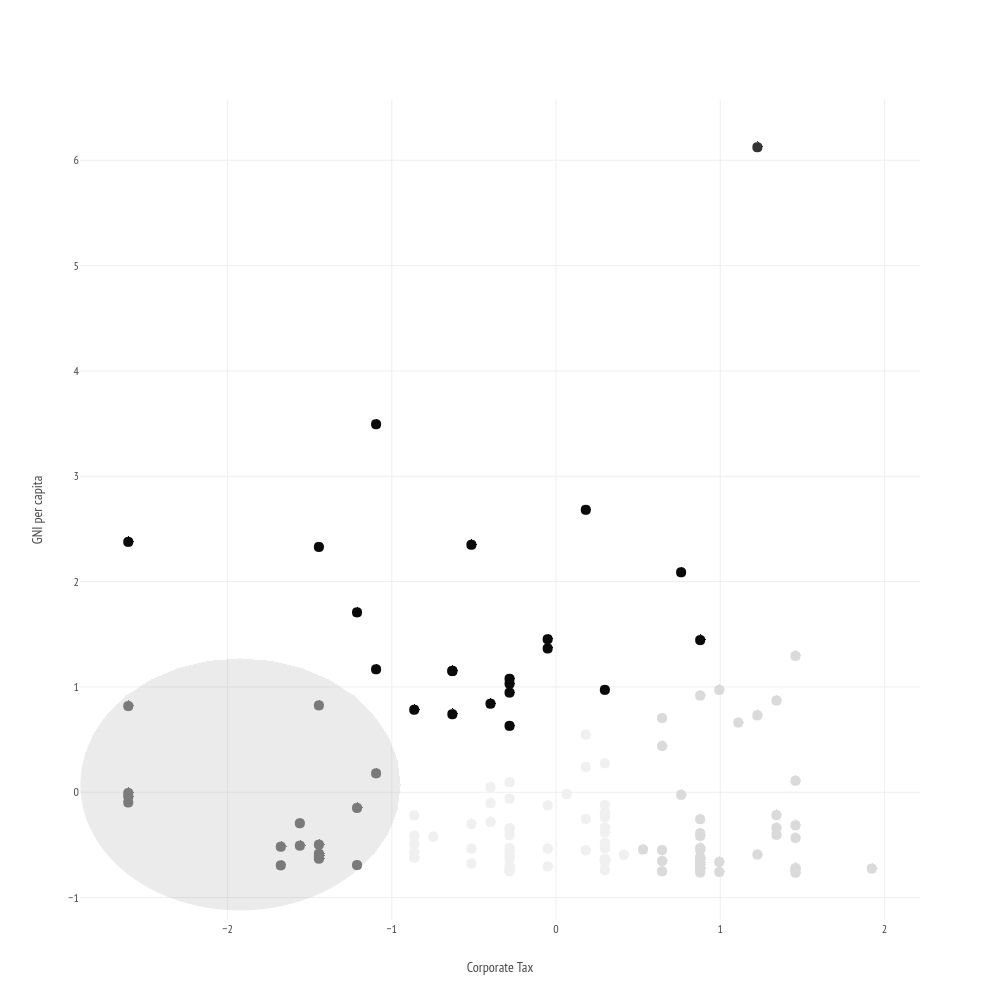
\includegraphics[width=1\linewidth]{Images/Cluster-GNI-CT.png}
\caption{K-mean cluster on standardized Corporate Tax and GNI per capita}
\end{figure}

\subsubsection{Target enterprise data}

This data includes the information from our enterprise (the one in which we're going to reallocate the entities). Even though, the data that can be extracted from the enterprise are enormous, the decision was to depict the most valuable information on the enterprise keeping under control the numerosity of such parameters. The parameter identified are: 
\begin{itemize}
	\item Revenues: they represent the upper limit that, whether crossed, our strategy will result not profitable, this element can be either forecasted or in case of a constant flow of revenues over the years, obtained through historical data;
	\item Employees: this element is somehow tied to the revenues expected, plus some limitations dictated by the labor unions depending by the countries (which were not modeled);
	\item Cost of running the asset: this is a very crucial factor in case of business that rely heavily on machinery and industrial plant activities, in fact such parameter may be neglected or, take a secondary position in the decision process, in case of a business relying heavily on employees, as for example a software company or a consulting firm.
\end{itemize}

While obtaining the first two parameters is something not particularly intensive in terms of data gathering and may require some additional effort the forecasting part because of the uncertainty that some industries carry. In case of the cost of running the assets two choices are proposed; it's possible to either use the internal data coming from a unified ERP system or use the single entity financial data and try to forecast each single entity cost of running the asset and then scale it to a common base in order to do an "apple to apple" comparison. In order to extract such parameter with the latter method the  operating expenses of the entity\cite{Williams2008} is used, subtracting from the operating expenses the wages the information inherent the cost of running the assets is obtained, the value is intended to be at a certain time $t_0$ for a certain volume of good $V_0$, dividing the cost of running the asset for $V_0$ will give a proxy of the marginal cost of asset given an increase of the production by one unit. This procedure has to be intended as measure of last resort in case of a non unified ERP system which still is the most reliable source of data in case of global entities located in very different countries. 
\\
\\
It's worth noting that are part of the enterprise data other information which are not part of the above mentioned parameters, such data deals with the DM preferences and some of them may involve limits in the numerosity of the number of entities. In some cases many enterprises can result in a trade off between potential synergies and the cost of keeping a constant flow of goods and information to them. This preference can narrow down till the functional characterization of an entity and may involve the localization in a particular country because of the public image of the Group.

\subsubsection{Global enterprises data}
This category contains all the data inherent the PLI of the specific functional enterprises operating in a certain State.
A piece of this data is summarized by the following representation. Another important data that can be obtained is the cost of debt \cite{Berman2013} even though such measure has to take into account the proportion of two types of funding (namely equity and debt) the data provided by the comparable enterprises serve as a good proxy for such measure if used in conjunction with financial databases as Bloomberg. In our case, to obtain this data a private worldwide database was used called Orbis by Bureau Van Dijk.

\begin{sidewaysfigure}
\centering
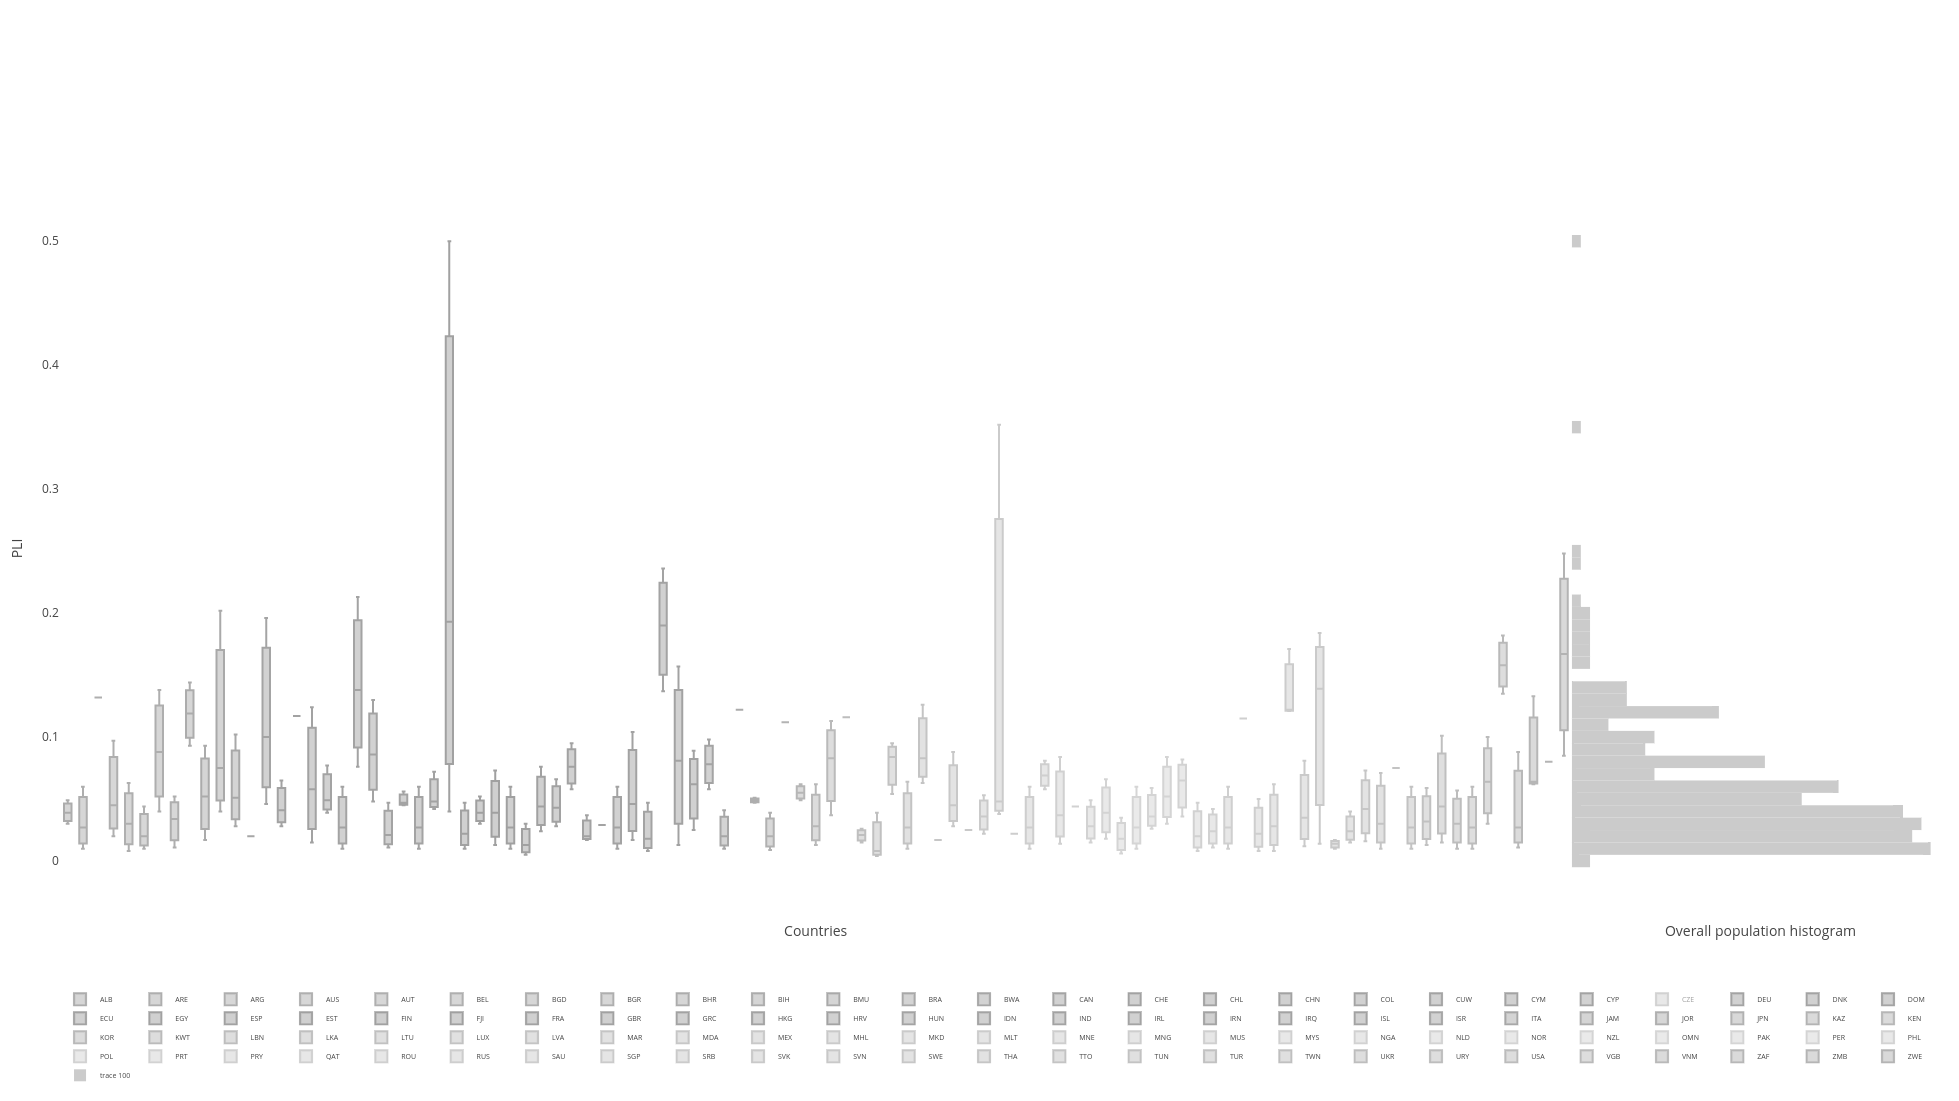
\includegraphics[width=\textwidth]{Images/plidist1.png}
\caption{Interquartile range of distribution PLI sorted by country}
\label{fig:interquartile}
\end{sidewaysfigure}

In the figure \ref{fig:interquartile}, is represented how the PLI interquartile range changes from country to country in such case the PLI chosen was an ROS applied on independent companies whose activities are  based on distribution (from wholesale to retail). Such difference can play a major role in deciding the optimal profitability level of the allocated entities. The PLI, acronym of Profit Level Indicator is the financial indicator (most of the time a ratio) that tracks the profitability of a certain function performed by the entity under scope of analysis.

\subsection{Objectives}
The data reported above will be used to set up the GP model and constitutes part of the objectives and constraints that will be presented below. In order to model the overall allocation the following objectives should be pursued:
\begin{itemize}
    \item The overall cost of production should be minimized;
    \item The tax liability should be minimized;
    \item The profit should be divided among the entities based on the contribution that such entity give to the overall process of value creation;
    \item The functional characterization of each entity must fall within a range achieved by comparable non controlled entities.
\end{itemize}

\subsubsection{Cost minimization}
This is a very basic objective in which the focus is to  minimize the cost embodied in each national entity. The cost function for each entity is primarily given by three variables, namely employees (which constitute the major variable cost of an enterprise) then the specific cost of running the assets (machinery, offices etc...) and ultimately the cost of capital (meaning the remuneration expected share holders and financiers). All these variables contribute to the determination of costs. The approximation function derived will look as follows:

\begin{equation}
C(E,A,K)=ce_k\cdot E+ca_k\cdot A+ck_k\cdot K \quad \forall k \in \left\{1...N\right\}
\end{equation}

Where 1.$ce_n$ corresponds to the National Income per Capita, this index was chosen because of its availability through the nations at scope and because it's a good proxy for the cost of labor in each State; 2.$ca_n$ corresponds to the cost of running the assets and is derived as illustrate before by subtracting the wage cost to the operational expenses and then adjusting for the purchasing power; 3.$ck_n$ corresponds to the cost of capital (in our case debt) calculated using data from comparable companies.
Even if this three variables do not represent the full cost structure of each enterprise (cost of good sold was not mentioned) is helpful for the decision maker to take into account this three driver of cost since this information constitutes the main driver to address value adding activities in the overall value chain.

\subsubsection{Tax base minimization}
This objective is the crucial point of this work since an optimal tax strategy can be considered good for profit maximization. However, should be mentioned that this doesn't constitute any avoidance of taxes but a strategy to be competitive in the market. Such allocation result in the consolidated minimization of all the national tax base, which is given by subtracting from the revenues allocated to a particular State ($y_k \cdot R$) the cost allocated to the same State (here expressed as $x_k \cdot C(E, A,K)$. This residual forms the EBIT (namely Earnings Before Interest and Taxes), the fraction of EBIT due to the tax authority is called the tax liability. The tax liability function will look as follows:

\begin{equation}
T(R,E,A,K)= [R-(ce_k\cdot E+ca_k\cdot A+ck_k\cdot K)]\cdot tx_k \quad \forall k \in \left\{1...N\right\}
\end{equation}

\subsubsection{Functional allocation}
This objective derives from the TNMM technique used in accessing the transfer pricing goodness. The method is based on the examination of the net profit relative to an appropriate base (e.g. costs, sales, assets) that a local entity realizes from a controlled transaction (or in our case to the entity itself). Basically, such objective works as a quality control that the overall process of maximization of profits as some confirmation also in the real market, made by independent actors. This is in certain sense a bond that helps the model in giving a solution viable also in an anti avoidance perspective.

In order to achieve this is necessary to identify which Profit Level Indicator to choose; this is an important choice that has to be made taking into account the functional characterization of such entity, that is, if an entity focuses on distribution the best PLI to test such entity is given by the ROS of its functional characteristics, that's because the sales are supposed to be the main element of a distributor (and not cost or assets). The main PLI used by practitioner are: Return on Sales, Full Cost Mark-up, Return on Asset, Return on Investment.

After each functional characteristic is matched with its relative PLI it's necessary to find the data of comparable independent entities, in order to asses the profitability range that our entity has to obtain to be in an arm's length position.

The objective function returning such objective would be as follows:

\begin{equation}
f(x) 
\begin{cases}
   \frac{R - C(E,A,K)}{R} & \text{if } q=1
   \\
   \frac{R - C(E,A,K)}{C(E,A,K)} & \text{if } q=2
   \\
   \frac{R - C(E,A,K)}{A} & \text{if } q=3
   \\
   \frac{R - C(E,A,K)}{E} & \text{if } q=4
\end{cases}
\end{equation}

The basic idea behind this objective is that for a moment we're forgetting about the group objective (the first and the second) that try to minimize the consolidated cost and tax base. In this case we're focusing on the profitability of each entity.

\subsection{Profit split}
This objective is represented by the goals (4e)(4f)(4g) and the methodology used to determine this type of split derives from the profit split method used in transfer pricing analysis. In particular the transfer pricing profit split aims at: determining the division of profits that independent enterprises would have expected to realize from engaging in the transaction \cite{OECD_ProfitSplit_2017}. In our case we'll use this method and particularly the contribution analysis to define the effort of each functional category in the value chain. Secondly we'll use this value driver to partition the profits in order to have, at the end, a structure that takes into account the internal value chain of the products and not just the information gained by independent comparable companies.


\subsection{Constraints}
Constraints represent the boundaries where the system will result unfeasible. Such constraints are expressed by the equation from (4h) to (4p); where the first two represent the boundaries on the PLI distribution namely the lower quartile and the upper quartile, outside this range the profitability may not be considered to be arm's length. The constraints (4j)(4k)(4l)(4m) represent the frontier of the possible allocable resources given by the company under the scope. The constraints (4n), (4o) and (4p) sets the positiveness of the deviation variables in order to avoid incorrectness of the overall GP model.

\subsection{Goal Programming Model}

This model aims to find the best allocation of costs and budgeted revenue in order to maximize profits minimizing costs and tax base, at the same time the model provides the best multinational functional allocation strategy to achieve such goal using both internal and external data from independent companies.
The objectives are divided into two categories; the first one is given by three objectives namely cost minimization, tax base minimization, PLI coherence; the second focuses more on the control and limitations that the decision maker wants to implement in the model due to the specific characteristics of its business.

The overall model algebraically looks as follows:

\begin{mini!}
  {p,n}{\sum_{i=1}^{Q} (\prescript{}{q}{p}_i \cdot w_i) + w_3 \cdot \sum_{i=1}^{O} (\prescript{}{o}{n}_i) + w_4 \cdot \sum_{i=1}^{N} ( \prescript{}{n}{n}_i + \prescript{}{n}{p}_i )}{}{}
	\addConstraint{\sum_{q=1}^{N} C_q(E,A,K) - \prescript{}{q}{p}_1}{=0}
	\addConstraint{\sum_{q=1}^{N} T_q(R,E,A,K) - \prescript{}{q}{p}_2}{=0}
	\addConstraint{P_k(R,E,A,K)+\prescript{}{n}{n}_k-\prescript{}{n}{p}_k}{=V_k,}{\forall k \in \left\{1...N\right\}}
	\addConstraint{\sum_{q=1}^{D} (R_q-C_q(E,A,K))+\prescript{}{o}{n}_1}{= c_1\cdot \sum_{q=1}^{N} (R_q-C_q(E,A,K))}
	\addConstraint{\sum_{q=1}^{P} (R_q-C_q(E,A,K))+\prescript{}{o}{n}_2}{= c_2\cdot \sum_{q=1}^{N} (R_q-C_q(E,A,K))}
	\addConstraint{\sum_{q=1}^{M} (R_q-C_q(E,A,K))+\prescript{}{o}{n}_3}{= c_3\cdot \sum_{i=q}^{N} (R_q-C_q(E,A,K))}
	\addConstraint{P_k(R,E,A,K)}{\geq L_k,}{\forall k \in \left\{1...N\right\}}
	\addConstraint{P_k(R,E,A,K)}{\leq U_k,}{\forall k \in \left\{1...N\right\}}
	\addConstraint{\sum_{q=1}^{N} R_q }{= R^*}
	\addConstraint{\sum_{q=1}^{N} E_q }{= E^*}
	\addConstraint{\sum_{q=1}^{N} A_q }{= A^*}
	\addConstraint{\sum_{q=1}^{N} K_q }{= K^*}
	\addConstraint{\prescript{}{q}{p}_i,\prescript{}{q}{n}_i}{\geq 0,}{i=1,...,Q}
	\addConstraint{\prescript{}{n}{p}_i,\prescript{}{n}{n}_i}{\geq 0,}{i=1,...,N}
	\addConstraint{\prescript{}{o}{p}_i,\prescript{}{o}{n}_i}{\geq 0,}{i=1,...,O}
\end{mini!}

Where the equations(4b)(4c)(4d) belong to the first category, where instead (4e)(4f)(4g) belong to the second, the latter in fact depend on the strategy of the decision maker and it's not given by any environmental variable.

\pagebreak

\section{Mathematical simulation: a case study}
The simulation of the above-mentioned model was made using LINGO17 and specifically its linear solver. Even if the mathematical package was able to handle the total amount of data given by the model the simulation was done using a portion of this data, avoiding countries in which the company doesn't operate at all. Other limitations were implemented in order to avoid any possible non-linearity, resulting in an increase of the computational time to obtain a solution, this was possible by avoiding inserting the equation (4d), when instead the correlated constraints, namely (4h) and (4i) were linearized. Other limitations of the model are exposed below:
\begin{itemize}
    \item The PLI chosen to set the functional range were only 2, ROS and FCMU;
    \item The cost of asset and equity was set to 0, meaning that the only cost driver was employees;
    \item The functional characterization was reduced to 3, namely distributor, producer and principal (which acts as an active holding);
    \item The number of employees was assumed to be continuous, meaning that part-time work and non full year worker can be used by the firm.
\end{itemize}

Concerning the data, the financials were taken from a company operating mostly in Europe and western countries in general, plus this company tend to produce and store most of its products in Asian countries and tend to have less inventory in its western distribution sites. The company under scope was underperforming at the time of this simulation its P/L statement registered a loss of roughly  6.000.000 USD. The revenues registered for the year under the scope were about 88.900.344 USD and the employees hired were 2.722.

\subsection{Sensitivity analysis}
In the sensitivity analysis, the value of the weights was preemptively determined; since the model for the case study has only three goals, namely the minimization of the operation cost, the minimization of the tax liability and conservation of the functional allocation. The aim of the sensitivity analysis was to measure all the possible frontiers between DM preference toward these choices. Therefore the objectives were subjected to different weights combination, however, the combinations didn't include any zero weight, this was done in order to avoid any Pareto solution that would result infeasible in reality. For the three objectives was given a set of possible weight alternatives following the equation reported below:
$$
1=x + y + z, \quad \forall x \in X, X = (0,1), \quad \forall y \in Y, Y = (0,1, \quad \forall z \in Z, Z = (0,1),
$$
Where $x$ is the preference for the minimization of the operational costs($w1$), whereas $y$ stands for the preference of the DM toward the minimization of the tax liability($w2$) and $z$ represents the preference for maintaining the functional characterization of the company($w3$).
In order to give a better perspective of these different set of preferences, a ternary plot was created representing some of the possible choice given admitted by the equation defined previously.

\begin{figure}[h]
\centering
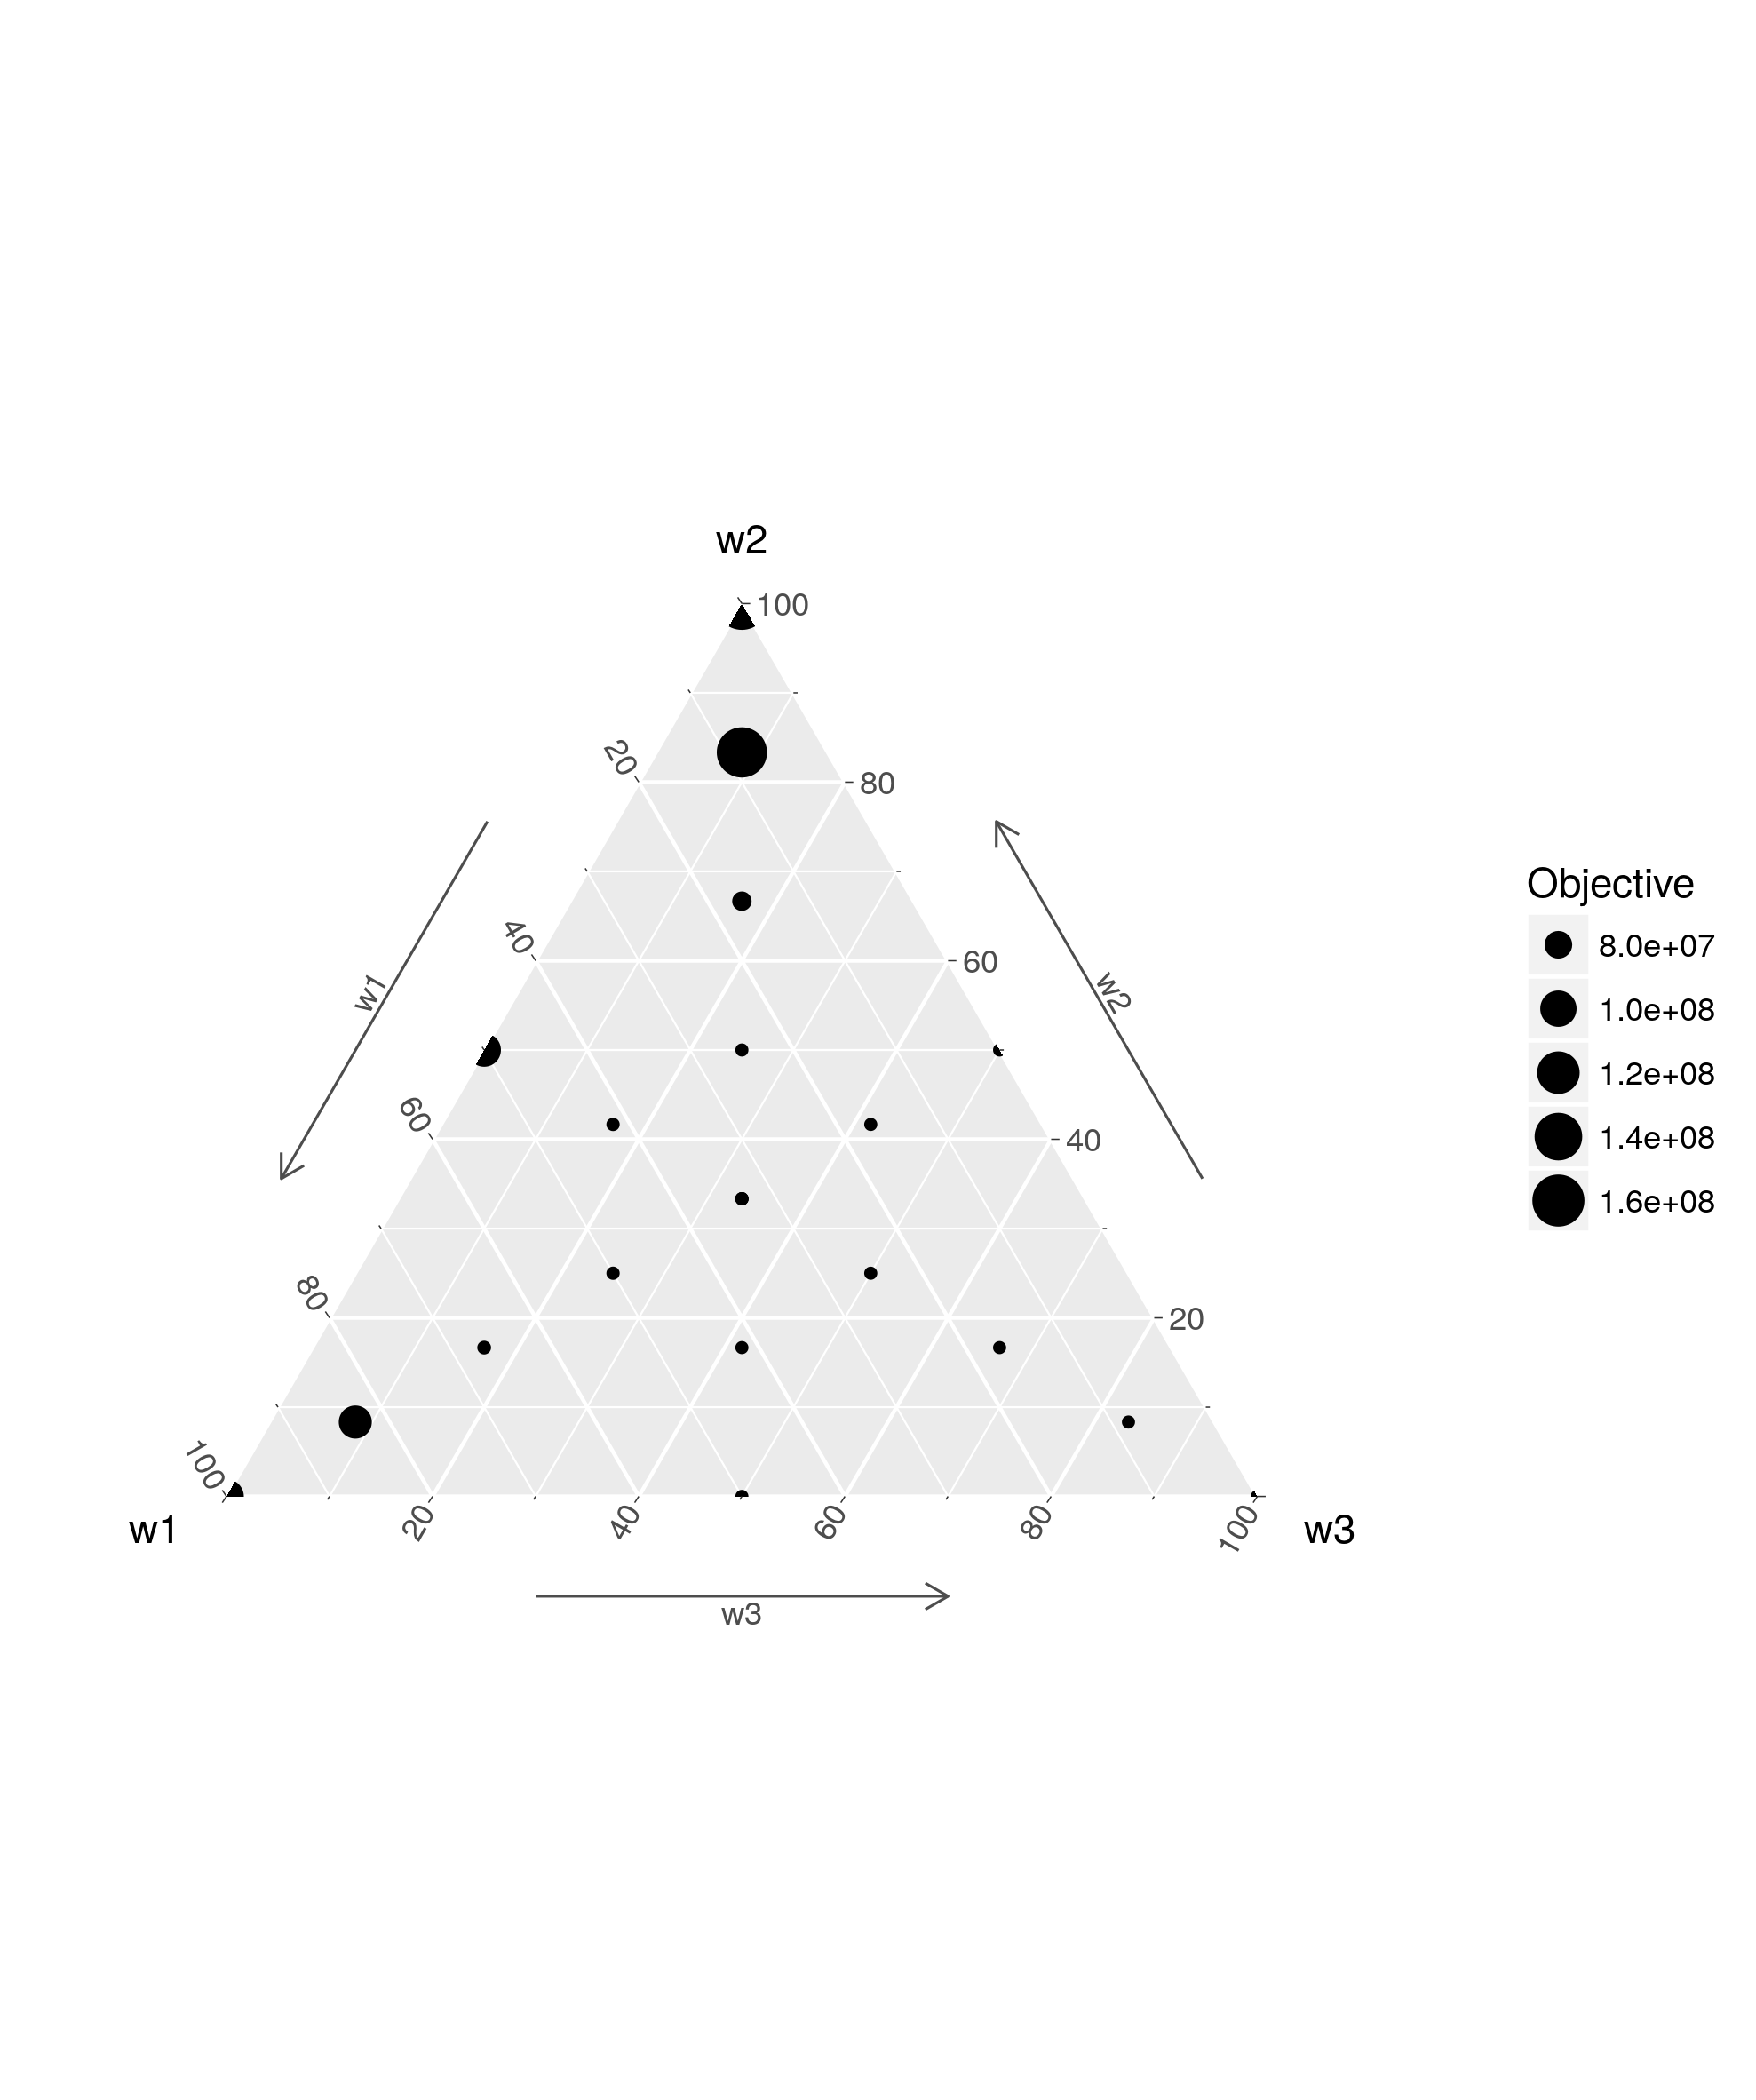
\includegraphics[width=0.7\linewidth]{Images/ternary.png}
\caption{Weight sensitivity analysis}
\end{figure}

As presented by the figure, pursuing largely the minimization of the operational cost could not be considered a great objective and the same as to be said by the sole objective of tax minimization, a much solid set of weights should be found taking into account these different outcomes.

\subsection{Analytical Hierarchical Process for weight determination}
Given the knowledge about the tradeoffs that DM faces, the option was to choose a robust framework to select the sensitivity of the weights that were consistent with the expectation that the Decision Maker has about the process of Green Supply Chain. The chosen framework was the Analytical Hierarchy Process \cite{Saaty1980}. The process was three tired:

\begin{itemize}
    \item Step 1: given the set of criteria defined in the previous sections the pairwise comparison matrix was computed indicating the importance of each criterion with respect to the other;
    \item Step 2: the pairwise matrix elements were normalized and consequently the priority vector was obtained;
    \item Step 3: the last step consists in the test of the consistency of the value reported and then the validation with respect to a randomly generated matrix consistency index.
\end{itemize}

The resulting table reports the pairwise comparison matrix pre normalization:

\begin{table}[ht]
\centering
\begin{tabular}{@{}llll@{}}
\toprule
\textbf{Criteria}     & Operation Costs & Tax Burden    & Functional Allocation \\ \midrule
Operation Costs       & 1.00            & 0.50          & 0.33                  \\
Tax Burden            & 2.00            & 1.00          & 0.50                  \\
Functional Allocation & 3.00            & 2.00          & 1.00                  \\
Total                 & \textit{6.00}   & \textit{3.50} & \textit{1.83}         \\ \bottomrule
\end{tabular}
\caption{Pairwise comparison matrix}
\end{table}

In the pairwise matrix is visible the preference of the DM toward maintaining the functional allocation above all other objectives. Subsequently the step 2 of the AHP method was followed, and then the normalized priority vector was obtained, which is represented in the table below.

\begin{table}[]
\centering
\begin{tabular}{@{}ll@{}}
\toprule
\textbf{Criteria}     & Weight        \\ \midrule
Operation Costs       & 0.16          \\
Tax Burden            & 0.30          \\
Functional Allocation & 0.54          \\
Total                 & \textit{1.00} \\ \bottomrule
\end{tabular}
\caption{Priority vector}
\end{table}

The order of importance was therefore functional allocation, followed by tax minimization and operational cost minimization. However, the resulting vector may be inconsistent because of different choices according to the tuples. Therefore the step 3 was necessary and a consistency check was made in order to assess the goodness of the priority vector.
The consistency ratio scored by the following preferences was $0.79\%$ and therefore accepted since the threshold suggested by Saaty\cite{Saaty1980} is $10\%$. Then the priority vector obtained was used to calibrate the weights of the model. After the calibration, the model was solved through the LINGO linear solver algorithm. The objectives achievement are reported in the table below.

\begin{table}[]
\centering
\begin{tabular}{@{}ll@{}}
\toprule
\textbf{Objective}    & Value         \\ \midrule
Operation Costs       & 26137120     \\
Tax Burden	      & 14798710     \\
Functional Allocation & 26134390     \\
Total                 & \textit{67070220} \\ \bottomrule
\end{tabular}
\caption{Objective value according to the model}
\end{table}

The solution is summarized in the figure \ref{fig:allocationmap}. The optimal solution was to create two different distribution entities namely one in India and one in Malta and keep the manufacturing in a country with a greater PLI (such as Denmark) because of the great margin between revenues and costs. The greater amount of this margin is possible to see in the principal function (located in Portugal) where this margin is increased because of the importance that such functions perform in the value chain. The solution proposed resulted in an average tax rate below the $20\%$.

\begin{sidewaysfigure}
\centering
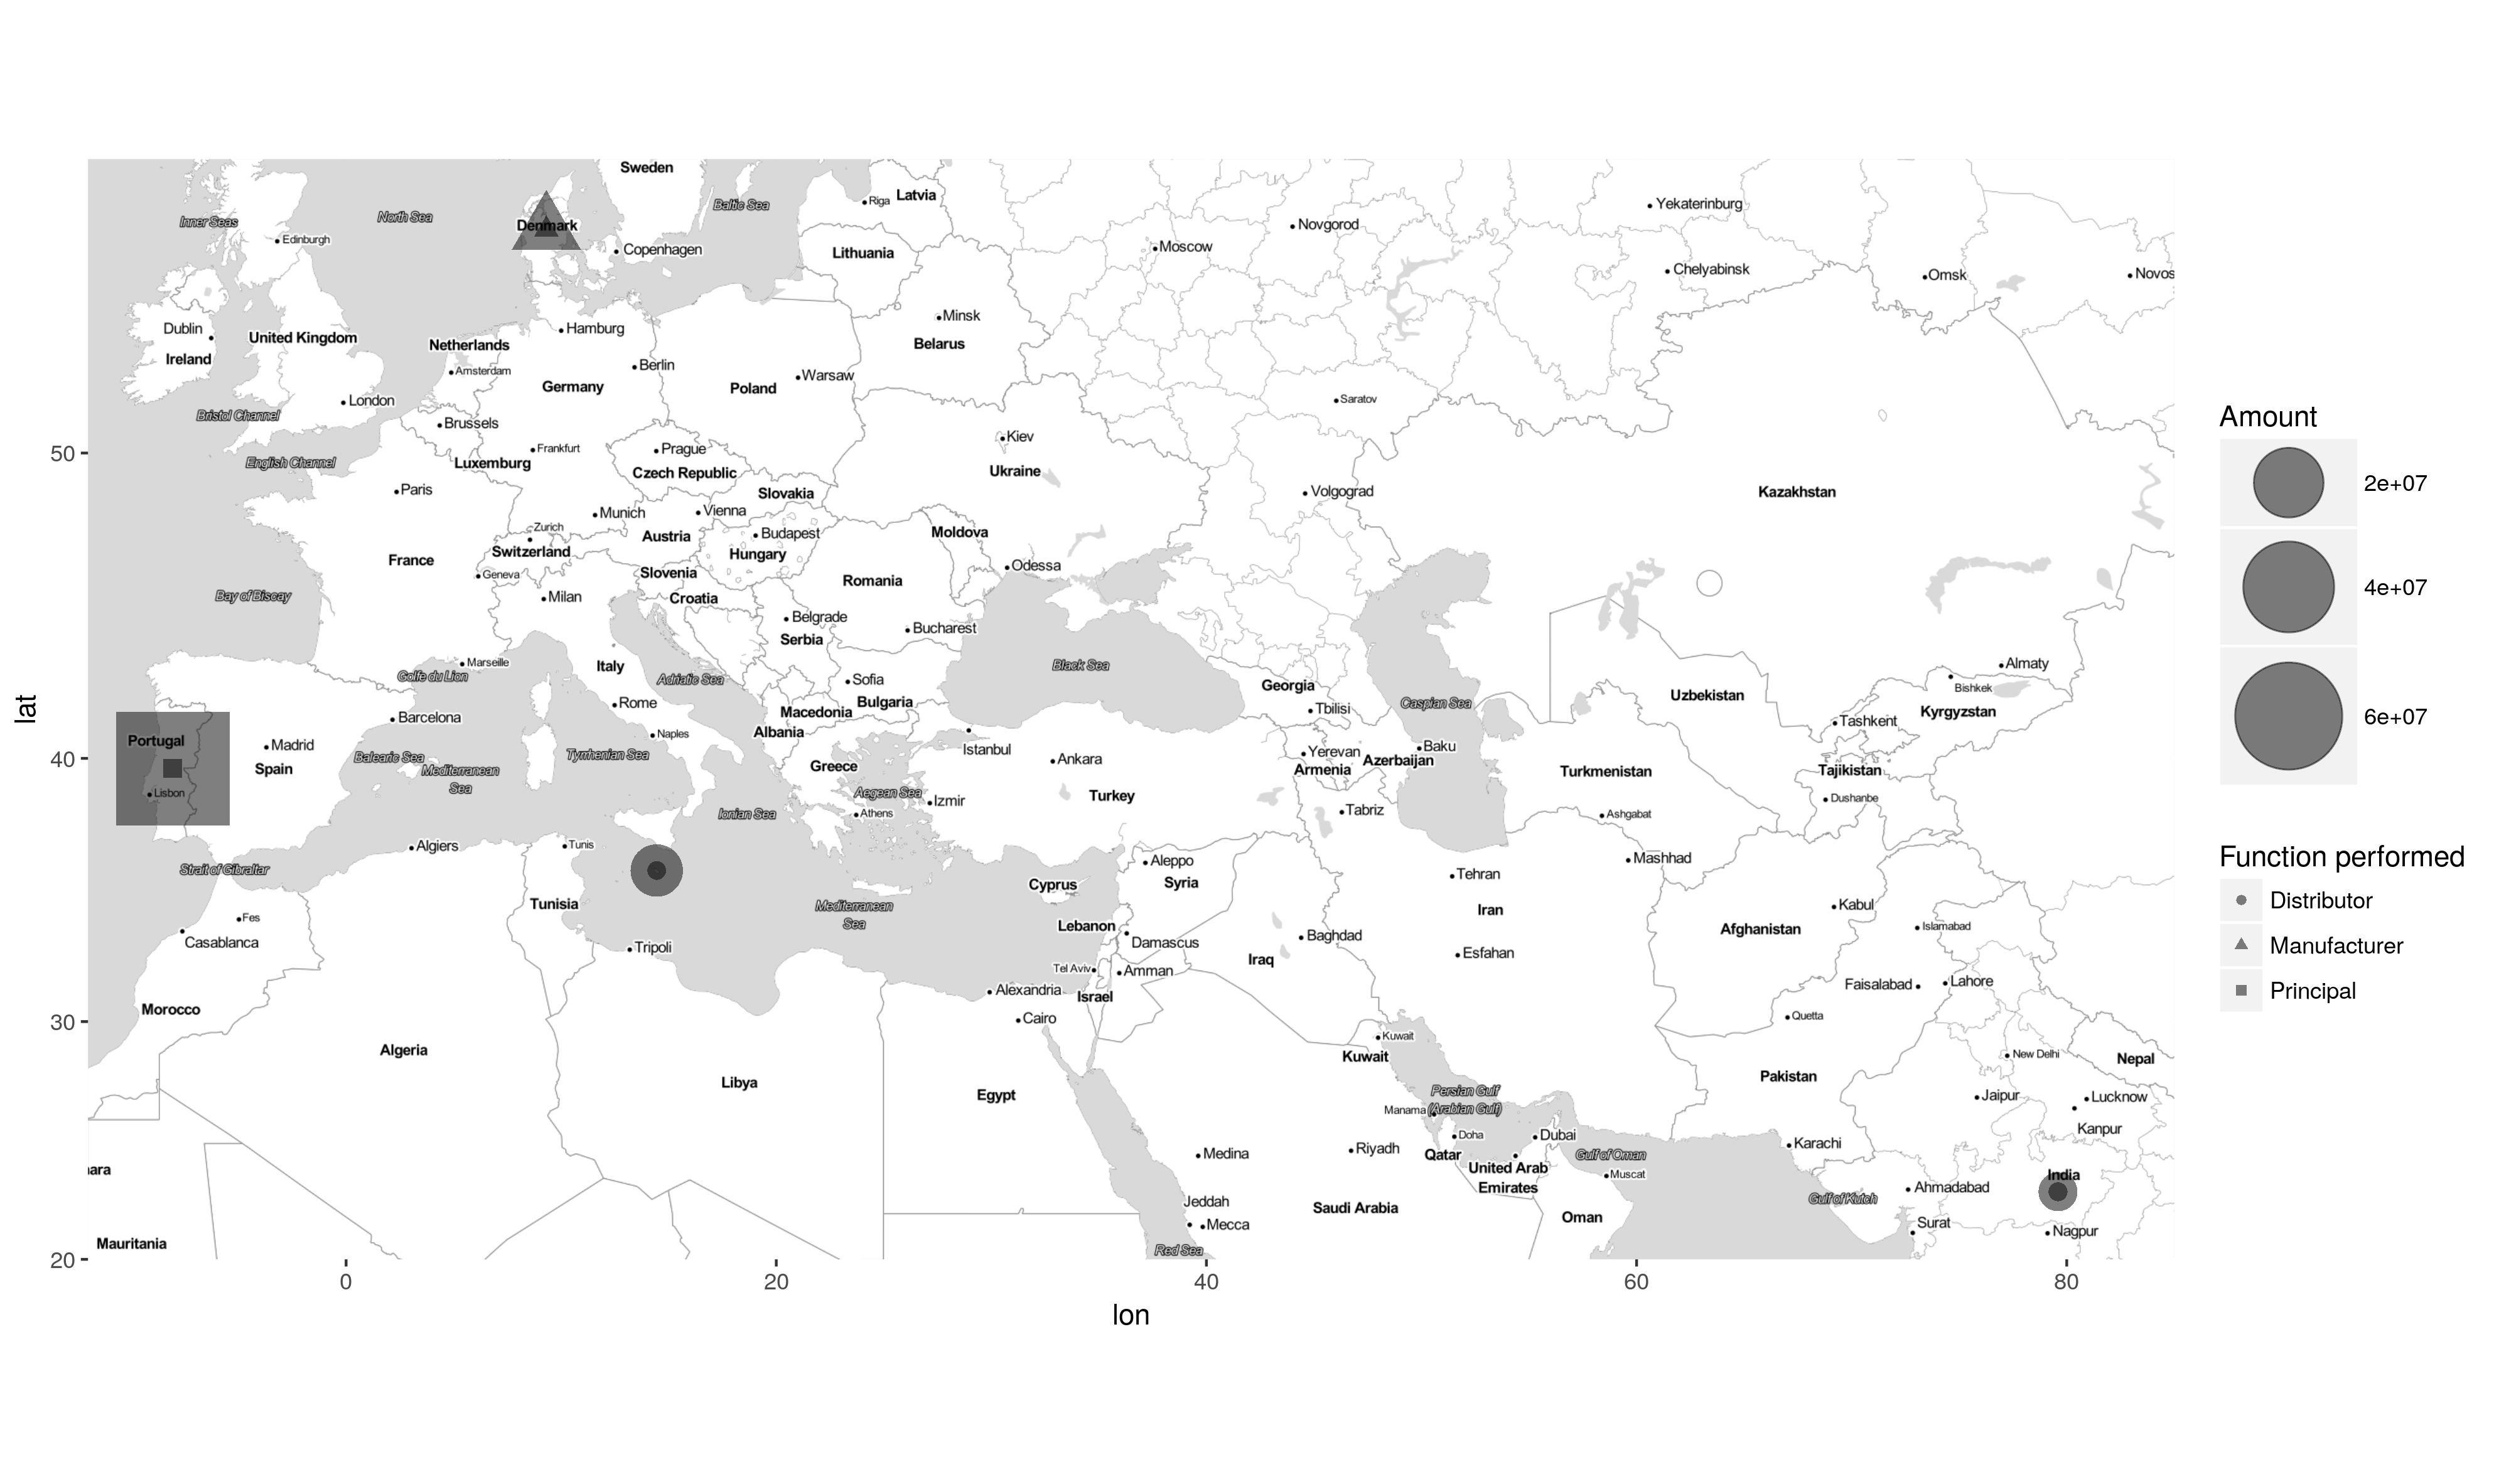
\includegraphics[width=\textwidth]{Images/AllocationMap.png}
\caption{Cost and revenues allocation according to the model}
\label{fig:allocationmap}
\end{sidewaysfigure}

\subsection{Final remarks}
The model proposed aims at seeking the optimal allocation of profits between the multiple multinational companies in order to be compliant with the transfer pricing regulation and with respect to the business carried by independent companies carrying similar functions. The lack of literature in the tax planning filed may be seen as a promising niche that researchers should pursue in the future. The model proposed apart from the simplistic assumption given in the case study could have been enhanced with other features belonging to the Goal Programming approach such as fuzzy sets to model the PLI range or other features. 
